
\documentclass[review]{elsarticle}

\usepackage{lineno}

\usepackage{amsmath}
\usepackage{amsfonts}
\usepackage{amsthm}
%\usepackage{url}
\usepackage{subfig}
\DeclareMathOperator*{\argmin}{argmin}
\newcommand*{\argminl}{\argmin\limits}
\newtheorem{prop}{Proposition}
\newtheorem{corollary}{Corollary}

\modulolinenumbers[5]

\journal{Statistics and Probability Letters}

%%%%%%%%%%%%%%%%%%%%%%%
%% Elsevier bibliography styles
%%%%%%%%%%%%%%%%%%%%%%%
%% To change the style, put a % in front of the second line of the current style and
%% remove the % from the second line of the style you would like to use.
%%%%%%%%%%%%%%%%%%%%%%% %% Numbered %\bibliographystyle{model1-num-names} %% Numbered without titles %\bibliographystyle{model1a-num-names} 
%% Harvard
%\bibliographystyle{model2-names.bst}\biboptions{authoryear}

%% Vancouver numbered
%\usepackage{numcompress}\bibliographystyle{model3-num-names}

%% Vancouver name/year
%\usepackage{numcompress}\bibliographystyle{model4-names}\biboptions{authoryear}

%% APA style
%\bibliographystyle{model5-names}\biboptions{authoryear}

%% AMA style
%\usepackage{numcompress}\bibliographystyle{model6-num-names}

%% `Elsevier LaTeX' style
\bibliographystyle{elsarticle-num}
%%%%%%%%%%%%%%%%%%%%%%%

\begin{document}

\begin{frontmatter}

\title{A Stopped Negative Binomial Distribution}
\tnotetext[mytitlenote]{This research was supported by grants R01CA131301, 
R01CA157749, R01CA148996, R01CA168733, and PC50CA196530 awarded by the 
National Cancer Institute along with support from the Yale Comprehensive Cancer 
Center and the Yale Center for Outcomes Research. We would also like 
to thank Rick Landin at Ignyta Inc. for his suggestions.}

%% Group authors per affiliation:
%\author{Elsevier\fnref{myfootnote}}
%\address{Radarweg 29, Amsterdam}
%\fntext[myfootnote]{Since 1880.}

%% or include affiliations in footnotes:
\author{Michelle DeVeaux}
\ead{michelle.deveaux@yale.edu}

\author{Michael J. Kane$^*$\footnote{* Corresponding author}}
\ead{michael.kane@yale.edu}

\author{Daniel Zelterman}
\ead{daniel.zelterman@yale.edu}

\address{Department of Biostatistics\\ School of Epidemiology and Public Health\\ Yale University, New Haven, CT}

\begin{abstract}
We introduce a discrete distribution suggested by curtailed
sampling rules common in early-stage clinical trials. We derive the
distribution of the smallest number of independent and identically
distributed Bernoulli trials needed to observe either $s$ successes 
or $t$ failures. This report provides a closed-form expression for the 
mass function and illustrates limiting approximations.
\end{abstract}

\begin{keyword}
discrete distribution\sep curtailed sampling
\end{keyword}

\end{frontmatter}

\linenumbers

\section{Introduction and Motivation}

Consider a prototypical early phase, single-arm clinical trial in which 
17 patients
are enrolled and treated. The binomial probability of a patient 
responding to treatment is $p=0.2$ 
under the null hypothesis that the treatment is not effective.
If seven or more patients out of these 17 respond to the treatment then we 
reject this hypothesis and the treatment is deemed successful at 
a significance level of $0.1$.  If fewer than seven respond then the null 
hypothesis is not 
rejected and the treatment is deemed ineffective.

If all 17 patients are enrolled at once, as in the classic
design, then the sample size is 17. However, in most clinical trials the
patients are enrolled sequentially over time.
In the present example, observing seven
successful patients is one endpoint and the number of enrollees required
could be as small as seven. Similarly 11
observed treatment failures also ends the trial. This sampling mechanism, in
which the experiment ends as soon as any predefined endpoint is reached, is
called {\em curtailed sampling}. Under curtailed sampling, the range of the
sample size for this trial is seven through 17.

Let us assume each patient outcome can be modeled as an independent,
identically distributed Bernoulli($p$) random variable. The trial is realized
as a sequence of Bernoulli samples stopping when either a
specified number of responders or non-responders has been reached. 

\begin{figure}[bp!]
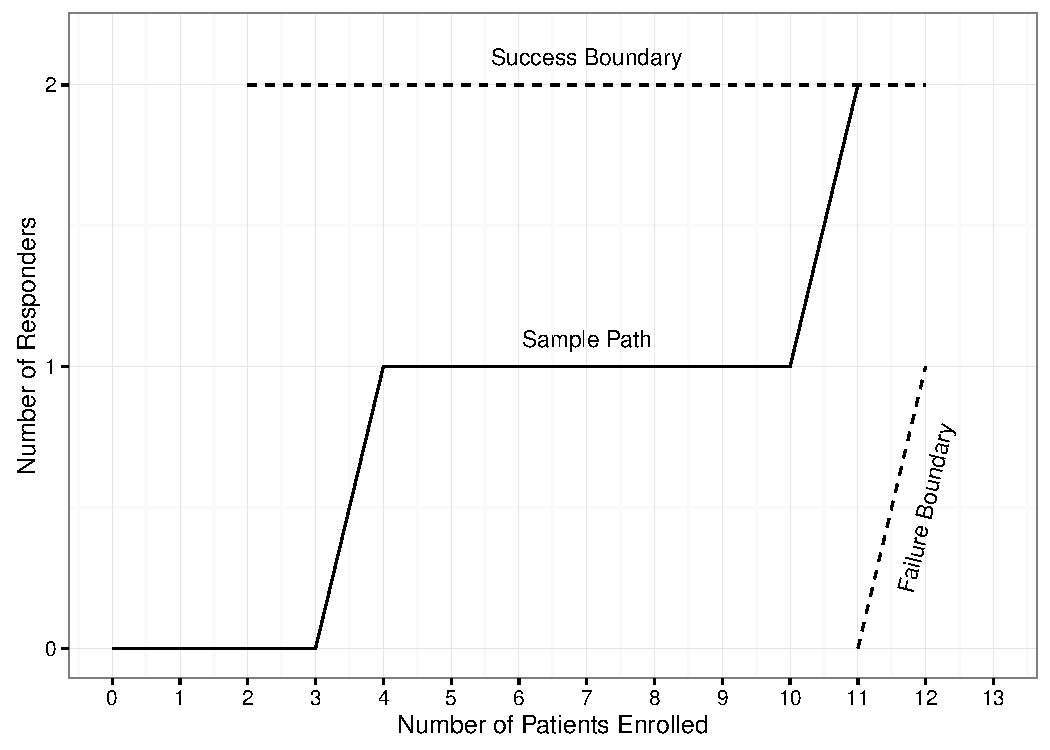
\includegraphics[width=\textwidth]{KanePlot.pdf}
\caption{
A hypothetical realization of the trial.
}
\label{fig:kane_viz}
\end{figure}

A hypothetical sample path is illustrated in Fig.~\ref{fig:kane_viz}.
The vertical axis denotes the number of
successful outcomes. The horizontal axis counts the number of patients 
enrolled. The horizontal and vertical boundaries represent
endpoints for the trial. In this case, a seventh response was reached on
the $15^{\text{th}}$ enrollment.
Since the success boundary is reached, we say the treatment succeeds.

%\begin{figure}[bp!]
%\centering
%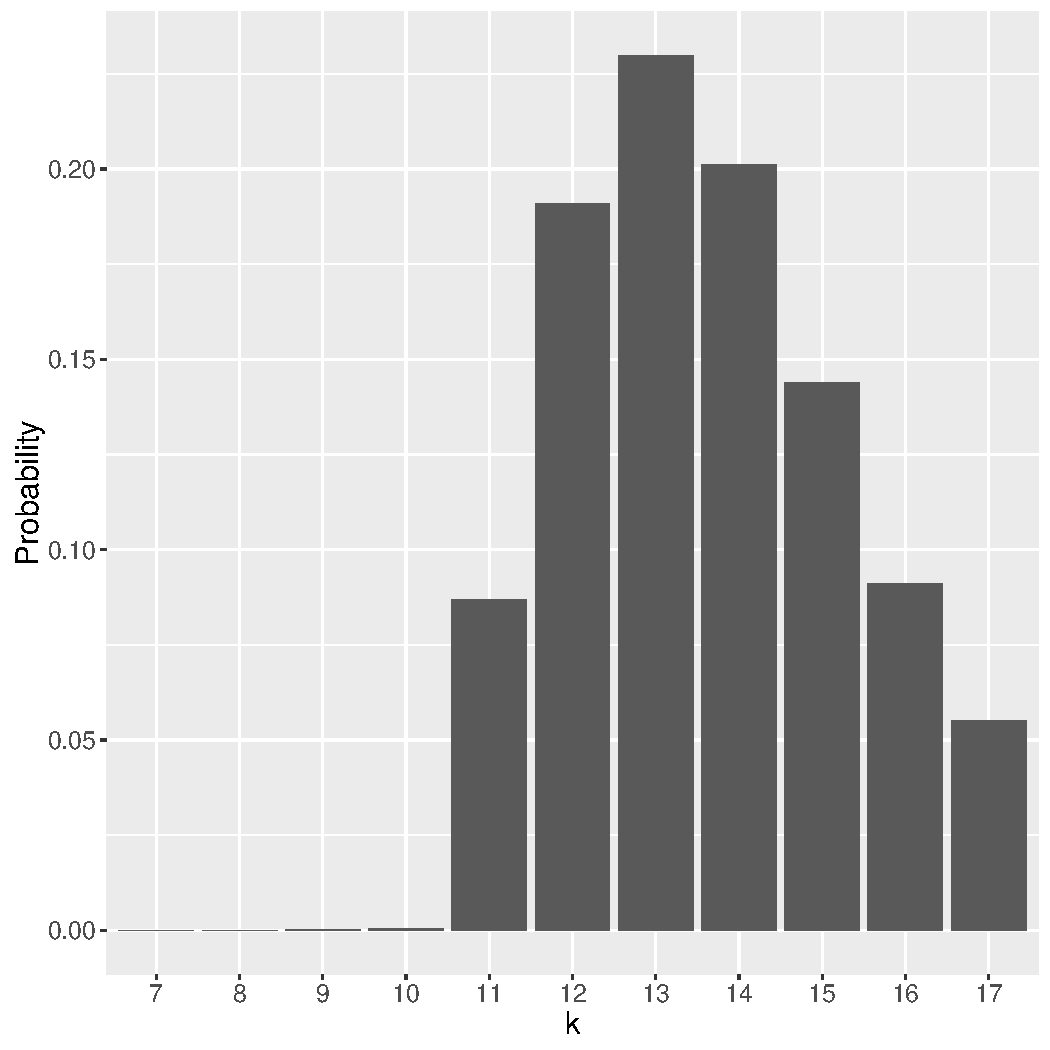
\includegraphics[width=\textwidth]{snb-first-plot.pdf}
%\caption{
%The probability mass function for a trial where $p$ 
%is 0.045 and where the trial stops
%after two patients respond or 11 patients do not respond.
%}
%\label{fig:first-plot}
%\end{figure}

\begin{figure}[bp!]
\centering
\subfloat[enrollment distribution]{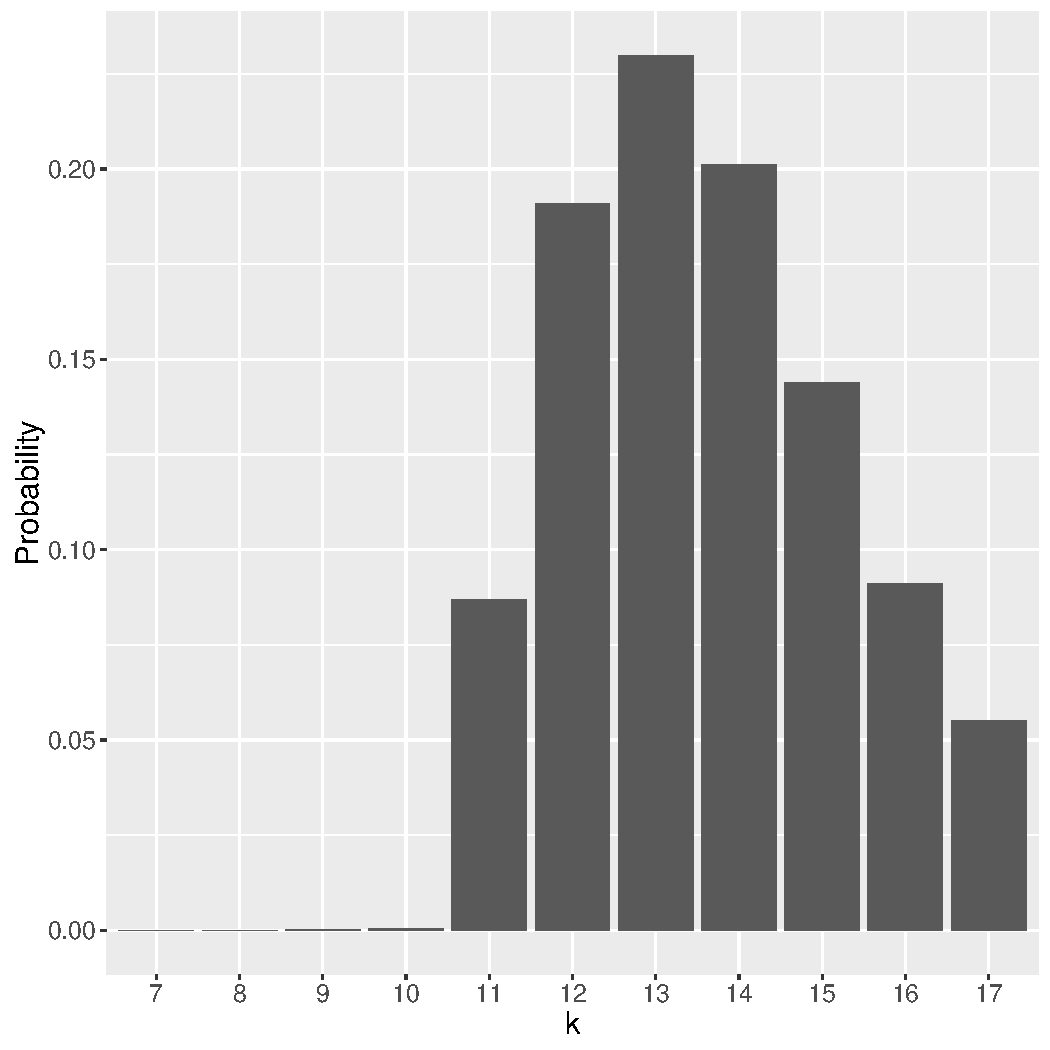
\includegraphics[width=0.5\textwidth]{snb-first-plot.pdf}}
\hfill
\subfloat[mean and variance varying $p$]{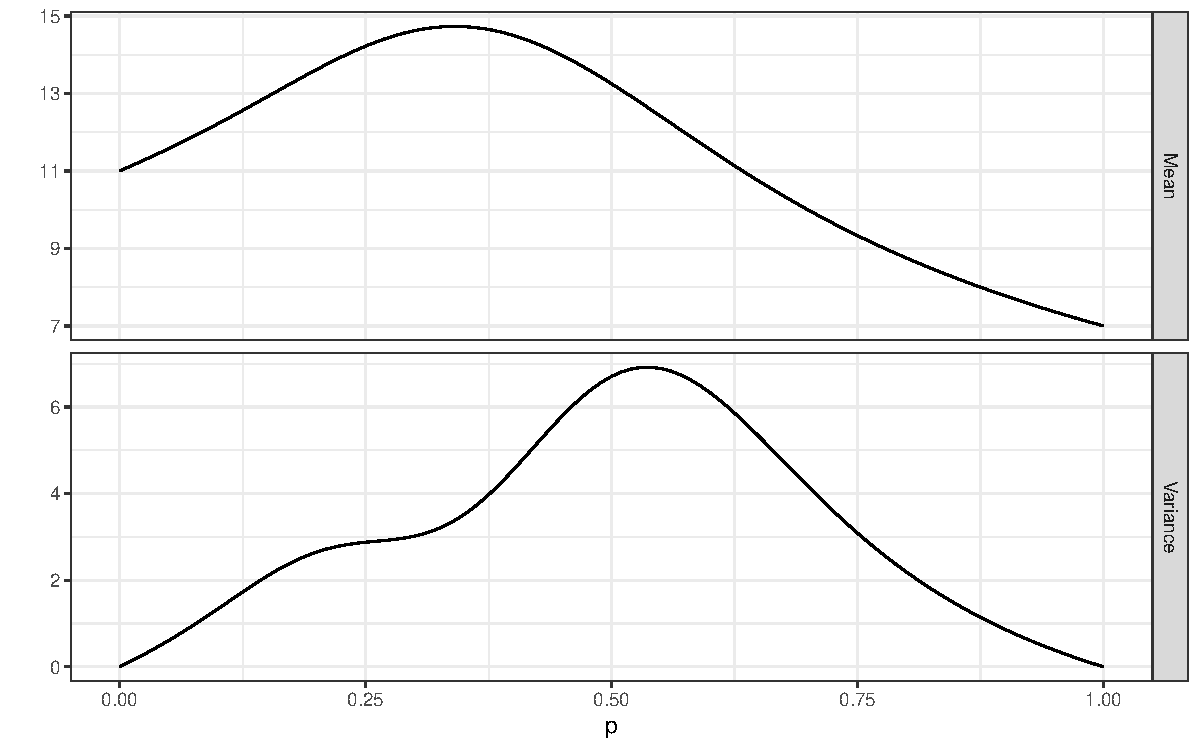
\includegraphics[width=0.5\textwidth]{mean-and-variance.pdf}}
\caption{
The distribution of a trial that stops after seven patients respond to treatment
or 11 patients do not. Panel (a) shows the distribution when
$p = 0.2$. The mean and variance of the distribution varying $p$ 
between zero and one are shown in panel (b).
}
\label{fig:exp-and-var}
\end{figure}

More generally the distribution of the number of trial enrollments is shown in 
Fig.~\ref{fig:exp-and-var} (a). There is relatively little probability mass
for values of sample size equal to seven through 10 since $p$ is small and it 
is unlikely the treatment will succeed quickly.
%The probability mass is concentrated at the 
%$11^{\text{th}}$ and $12^{\text{th}}$ step since $p$ 
%is small and for most realizations reach 11 
%non-responders before reaching 2 responders.
Fig.~\ref{fig:exp-and-var} (b) shows the expected value and variance for the
number of trial enrollments varying $p$ between zero and one. When $p$ is
small then the treatment
is more likely to fail shortly after the $11^{\text{th}}$ enrollment.
When $p$ is large then the treatment is more likely to succeed and the 
number of enrollees approaches seven from above. 

When $p=0$ or $1$ the processes are deterministic and variance is zero.
Values between zero and one change the mixing proportions of 
the two endpoints. The saddle around $p=0.25$ results from inequality 
in the size of the support of the two endpoints.

%\begin{table}[t!]
%\caption{Characteristics of the Stopped Negative Binomial Distribution}
%\label{tab:snb}
%\begin{center}
%\begin{tabular}{|c|l|} \hline
%Parameters & $p$ the success probability ($0\leq p \leq 1$; $q = 1-p$) \\
%           & $s$ the number of successes before stopping ($s=1, 2, ...$)\\
%           & $t$ the number of failures before stopping ($t=1, 2, ...$)\\ \hline
%Support & min$(s,t) \leq k \leq s+t-1$  \\ \hline
%$\mathbb{P}[Y=k]$ & ${k-1 \choose s-1} p^s (1-p)^{k-s} I_{\{s \leq k \leq s+t-1\}\}}+ {k-1 \choose t-1} (1-p)^s p^{k-t} I_{\{t \leq k \leq s+t-1\}}$\\ \hline
%$\mathbb{P}[Y \leq k]$ & $2 - \mathcal{I}_{q}(k+1, s) - \mathcal{I}_{p}(k+1, t)$\\ 
%    & where $\mathcal{I}$ is the regularized incomplete beta function.\\ \hline
%Mean & $\frac{s}{p} \mathcal{I}_p(s,t) + \frac{p^{s-1} q^{t-1}}{B(s,t)} +
%  \frac{t}{q} \mathcal{I}_q(t,s) + \frac{p^{t-1} q^{s-1}}{B(s,t)}$\\ 
%  & where $B$ is the beta function \\ \hline
%MGF & $\left(\frac{p e^x}{1 - qe^x}\right)^s 
%  \mathcal{I}_{1-qe^x} (s, t) + \left(\frac{qe^x}{1-pe^x}\right)^t 
%  \mathcal{I}_{1-pe^x}(t, s) $\\ \hline
%Predictive Distribution & 
%${k-1 \choose s-1} \frac{B\left(\alpha+s, k-s+\beta \right)}{B(\alpha, \beta)}+
%{k-1 \choose t-1} \frac{B\left(\alpha + k-t, t+\beta\right)}{B(\alpha,\beta)}$\\
%& for $p$ distributed as Beta($\alpha$, $\beta$). \\ \hline
%\end{tabular}
%\end{center}
%\end{table}

In the rest of this work, we derive the distribution of the number of 
enrollees needed
to observe either $s$ successes or $t$ failures. We refer to this distribution
as the Stopped Negative Binomial (SNB). 
%Some of its characteristics are summarized in Tab.~\ref{tab:snb}.
This paper derives this distribution and explores its properties.
%The next section introduces our notation and basic results
%including the density of the distribution along with a description of
%its relation to other distributions. 
Section 2 derives the distribution function
based on a defined Bernoulli process and gives some basic properties.
Section 3 shows how the distribution is related to other standard
distributions and connects the SNB tail probability to the binomial tail 
probability.
Section 4 derives the moment generating function.
Section 5 derives the predictive and posterior distributions when $p$ has a 
beta prior distribution.

\section{Probability Mass Function}
\label{notation.section}

Let $\,b_1, b_2, \ldots \,$ denote a sequence of independent, identically
distributed, Bernoulli random variables with $\mathbb{P}[b_i=1]=p$ and
$\mathbb{P}[b_i = 0] = 1-p$, for
probability parameter $0\leq p \leq 1$. In the clinical trial setting
$\,b_i = 1$ corresponds to a patient responding to treatment.  
Let $s$ and $t$ be positive integers.  Define the SNB random
variable $Y$ as the smallest
integer value such that $\,\{b_1, \ldots , b_Y\}\,$ contains {\em either}
$\,s\,$ responders {\em or} $\,t\,$ non-responders. That is, the SNB 
distribution of $Y$ is the smallest integer such that either
$\sum_i^Y b_i = s$ or $\sum_i^Y 1-b_i = t$.

The distribution of $\,Y\,$ has support on integer values in the range
\begin{equation*}               
     \min(s,t) \leq \; Y \;\leq s+t-1  \label{range.y.eq}.
\end{equation*}
The probability mass function is
\begin{equation} \label{eqn:pmf}
\mathbb{P} [Y=k] = S(k, p, s) \ I_{\{s \leq k \leq s+t-1\}} + 
  S(k, 1-p, t) \ I_{\{ t \leq k \leq s+t-1 \}}
\end{equation}
where $I_{\{f\}}$ is the {\em indicator function}, taking the value 
of one if $f$ is true and zero otherwise, and
\begin{equation} \label{eqn:N}
S(k, p, s) = {k-1 \choose s-1} p^s (1-p)^{k-s} 
\end{equation}
is the negative binomial probability mass.

To prove (\ref{eqn:pmf}), consider the
process $\mathbf{X} = \left\{X(k) : k = 0,1,... \right\}$
with $X(0)=0$ and
\begin{equation*} \label{eqn:proc}
X_{k+1} = X_k + b_{k+1} \ I_{\{ k-t < X_k < s\}}.
\end{equation*}
At each step a patient's outcome is measured. In Fig.~\ref{fig:kane_viz} 
we consider a graphical illustration of the plot $X_k$ against
$k$. If the outcome of the $k$th patient responds to treatment then the process 
advances diagonally in the positive horizontal and vertical direction. 
If the $k$th patient does not respond
then the sample path advances in the positive horizontal direction only. The
process continues until either $X_k = s$ or $X_k = k-t$ corresponding to the
success and failure boundaries in Fig. \ref{fig:kane_viz}, respectively.

\begin{prop}
The distribution of the stopping time
\begin{equation*}
Y = \argminl_k \left[X_k \geq s \cup X_k \leq k-t \right]
\end{equation*}
is given at (\ref{eqn:pmf}).
\end{prop}
\begin{proof}
%The proof will proceed in two parts. First, a combinatorial justification 
%will be given for the probability mass value on each element of the support. 
%Second, it will be shown that the sum of the masses over the support sums to 
%one.

The probability a given realization of $\mathbf{X}$ reaches $s$ at
the $k$th outcome is the probability that, at time $k-1$, there are $s-1$
successful outcomes and $k-s$ unsuccessful outcomes multiplied by
the probability of a final success at time $k$. This expression is given
in (\ref{eqn:N}). 
Similarly, the probability a given realization reaches $k-t$
is the probability that, at outcome $k-1$, there are $k-t$ successful outcomes
and $t-1$ unsuccessful outcomes multiplied by the probability of a final
unsuccessful outcome at time $k$.  

%Next, define
%\begin{equation} \label{stop_t}
%S'(k, p, t) = {k-1 \choose k-t} p^{k-t} (1-p)^t
%\end{equation}
%and notice that $S(k, p, s) = S'(k, 1-p, s)$ by writing
%\begin{equation*}
%{k-1 \choose k-s} = {k-1 \choose s-1}.
%\end{equation*}

To show that (\ref{eqn:pmf}) sums to one, define
%\begin{align} \label{eqn:sum_proof}
%R &= \sum_{k=s}^{s+t-1} S(k, p, s) + \sum_{k=t}^{s+t-1} S(k, 1-p, t) \\
%  &= \sum_{k=s}^{s+t-1} {k-1 \choose s-1} p^s (1-p)^{k-s} + \sum_{k=t}^{s+t-1} {k-1 \choose k-t} p^{k-t} (1-p)^t
%\end{align}
\begin{equation*} 
R = \sum_{k=s}^{s+t-1} S(k, p, s) + \sum_{k=t}^{s+t-1} S(k, 1-p, t).
\end{equation*}
If we substitute $i=k-s$ in the first summation and $j=k-t$ in the second then
$R$ can be written as the cumulative distribution function of two
negative binomial distributions:
\begin{equation} \label{eqn:transformed_sum}
R = \sum_{i=0}^{t-1} {i+s-1 \choose i} p^s (1-p)^i \; + \;
\sum_{j=0}^{s-1} {j+t-1 \choose j} p^j (1-p)^t.
\end{equation}

Let $\mathcal{I}_p(s, t)$ be the {\em regularized incomplete beta function} 
\citep{Olver2010}. This function satisfies 
$\mathcal{I}_p(s, t) = 1-\mathcal{I}_{1-p}(t, s)$ \citep{Uppuluri1967}. Then
\begin{align*}
R = \sum_{i=0}^{t-1} &{i+s-1 \choose i} p^s (1-p)^i +
\sum_{j=0}^{s-1}  {j+t-1 \choose j} p^j  (1-p)^t \\
   &= 1-\mathcal{I}_p(s, t) + 1 - \mathcal{I}_{1-p}(t, s) \\
   &= 1. 
\end{align*}
This completes the proof that (\ref{eqn:pmf}) is the distribution of the
stopping time and is a valid probability mass function.
\end{proof}

Next, we consider an interim analysis of a clinical trial after $s'$ 
patients respond to treatment 
and $t'$ fail to respond for $s' < s$ and $t' < t$.
\begin{corollary} \label{conditional_distribution}
The number of subsequent enrollments needed 
to reach either $s$ or $t$ endpoints behaves as SNB($p$, $s-s'$, $t-t'$).
\end{corollary}
Having observed $s'$ responders and $t'$ non-responders, there are $s-s'$ 
more responders needed to reach the success endpoint and $t-t'$ more 
non-responders needed to reach the failure endpoint.

\section{Connections and Approximations to Other Distributions}

\begin{figure}[p!]
\begin{center}
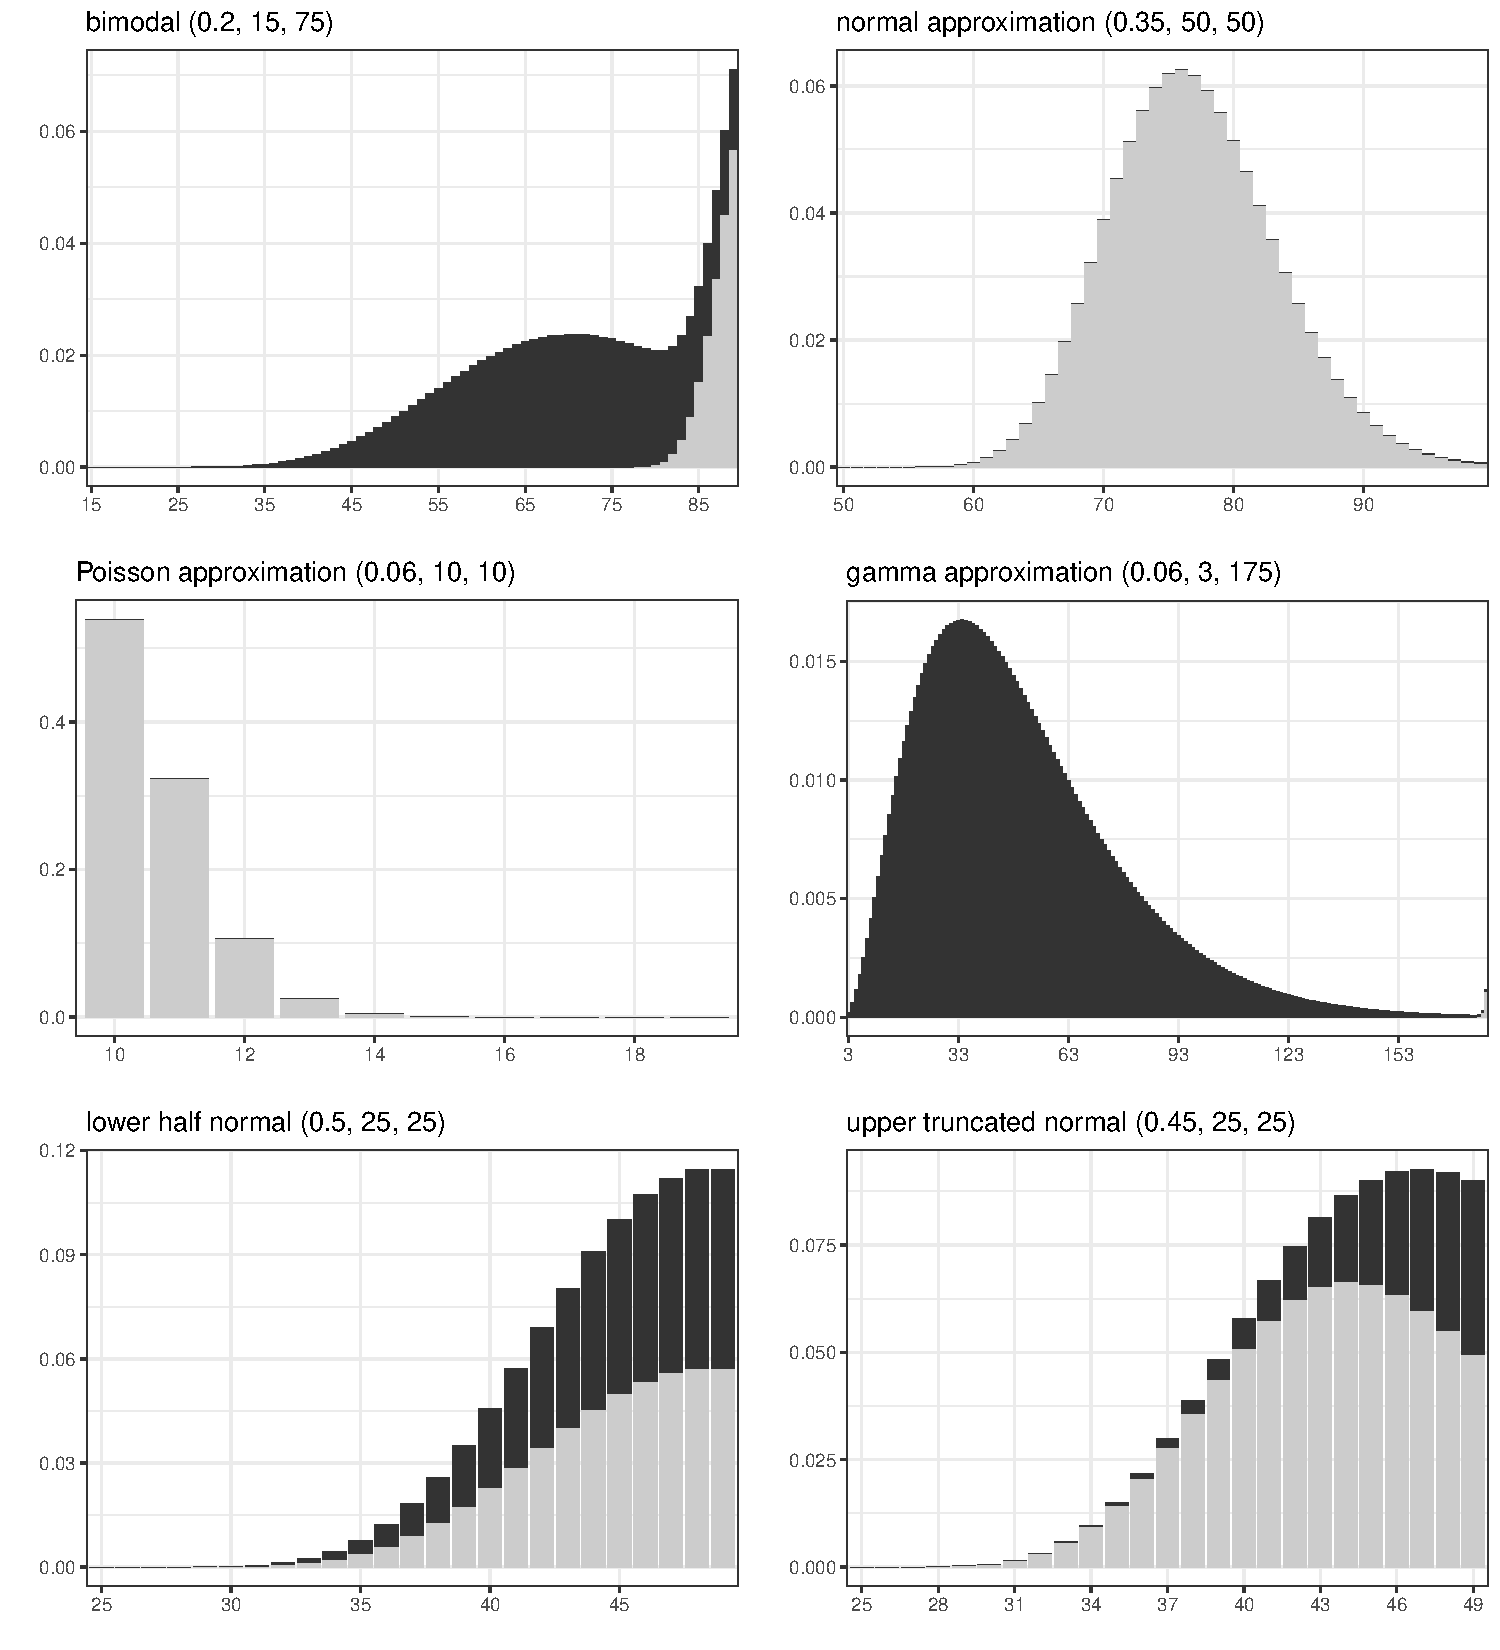
\includegraphics[width=\textwidth]{shapes.pdf}
\end{center}
\caption{Different shapes of the SNB distribution with parameters 
($p$, $s$, $t$), as given. Black indicates mass contributed by reaching
$s$ responders before $t$ non-responders. Grey indicates
mass contributed by reaching $t$ non-responders first. \label{shapes.fig}}
\end{figure}

The SNB is a generalization of the negative 
binomial distribution. When $t$ is large then $Y-s$ has a 
negative binomial distribution with
\begin{equation*}                                    %   (1)   
\mathbb{P}[Y=s+j\ |\ t \text{ is large\ }]        \label{nb1.eq}          
  = {{s+j-1}\choose{s-1}} p^s (1-p)^j
\end{equation*}
for $\,j=0, 1,\ldots\,$. A similar statement can be made when $s$ is large
and $t$ is moderate. As a result, with proper parameter choice, the SNB
can mimic other probability distributions in a manner similar to 
those described in \cite{Peizer1968} and \cite{Best1974}. Examples are
shown in in Fig.~\ref{shapes.fig}. 

The SNB generalizes both the minimum (riff-shuffle) and maximum negative
binomial distributions up to a translation of the support.
For the special case of $\,s=t,$ the distribution of $\,Y\,$ is the
riff-shuffle, or minimum negative binomial 
distribution~\citep{Uppuluri1967,Johnson2005}.
The maximum negative binomial \cite{Zhang2000,Zelterman2005,Johnson2005} is 
the smallest number of outcomes necessary to 
observe at least $s$ responders {\em and} $s$ non-responders and is equivalent
to a translated version of the riff-shuffle. 

%\section{Connection Between the SNB and the Binomial Tail Probability}

%There is a close connection between the tail probabilities of the SNB and the 
%binomial distributions.
%The probability of reaching the success endpoint in an 
%SNB($p$, $s$, $t$) random variable is 
%equal to the probability of at least $s$ successes in a binomial distributed 
%random variable with size $s+t-1$ and success probability $p$. 
%Likewise, the probability of reaching the failure endpoint is equal
%to the probability of at most $s-1$ successes in a binomial distribution. 
There is an equivalence between the probability of reaching an endpoint 
in the SNB model and the tail probability of the binomial distribution.
That is, the probability that the number of responders is at least $s$ in the 
binomial model is the same as the probability the treatment succeeds 
(reaches $s$) in the SNB 
model.
\begin{prop} \label{binomial_tail}
Let $Y$ be distributed as SNB($p$, $s$, $t$) and let $X_Y$ correspond
to the number of responders at the end of the trial. Let 
$B$ be distributed binomial with size $n=s+t-1$ and response probability
$p$. Then
\begin{equation}
\mathbb{P}[B \geq s] = \mathbb{P} [X_Y = s].
\end{equation}
\end{prop}
\begin{proof}
The binomial tail probability is
\begin{equation*}
\mathbb{P}[B \geq s] = 1 - \mathcal{I}_{1-p}(s, t)
\end{equation*}
%\begin{align*}
%\mathbb{P}[B \geq s] &= \sum_{k=s}^{s+t-1} {n \choose k} p^k (1-p)^{n-k} \\
%  &= 1 - \sum_{k=0}^{s-1} {n \choose k} p^k (1-p)^{n-k} \\
%  &= 1 - \mathcal{I}_{1-p}.
%\end{align*}
where $\mathcal{I}_{1-p}(s, t)$ is the {\em regularized incomplete beta} 
function. The corresponding success probability is
\begin{equation} \label{eqn:success}
\mathbb{P} [X_Y = s] 
  = \sum_{k=s}^{s+t-1} {k-1 \choose s-1} p^s (1-p)^{k-s}.
\end{equation}
Let $i=k-s$. Since
\begin{equation*}
{i+s-1 \choose s-1} = {i+s-1 \choose i},
\end{equation*}
the summation in (\ref{eqn:success}) can be rewritten as
\begin{align*}
\mathbb{P} [X_Y = s] &= \sum_{i=0}^{t-1} {i+s-1 \choose i} p^s (1-p)^i\\
  &= 1 - \mathcal{I}_{1-p}(t, s)
\end{align*}
completing the proof.
\end{proof}

To illustrate this result, let us return to our initial example
where $s=7$, $t=11$, and $p=0.2$.  The probability masses in
Fig.~\ref{fig:snb_bin_compare} represented in 
black are equal in panels (a) and (b) as are the masses in grey.
The probability that $s$
responders are reached in the SNB process is the same as the binomial 
probability of at least seven responders. Likewise, the probability that $t$ 
non-responders are reached in the SNB process is the same as the binomial
probability of zero through six responders.

\begin{figure}[t!]
\centering
\subfloat[SNB distribution]{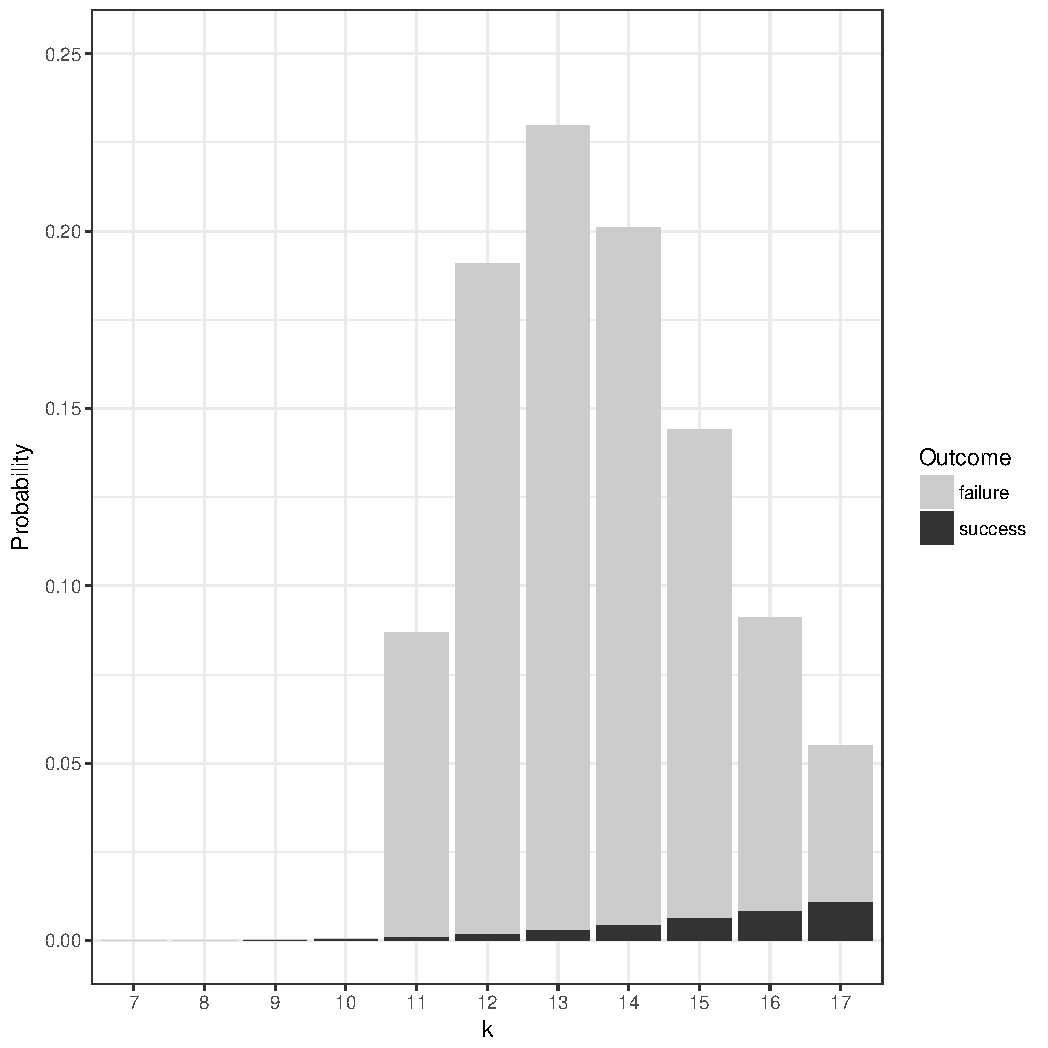
\includegraphics[width=0.5\textwidth]{snb_density.pdf}}
\hfill
\subfloat[binomial distribution]{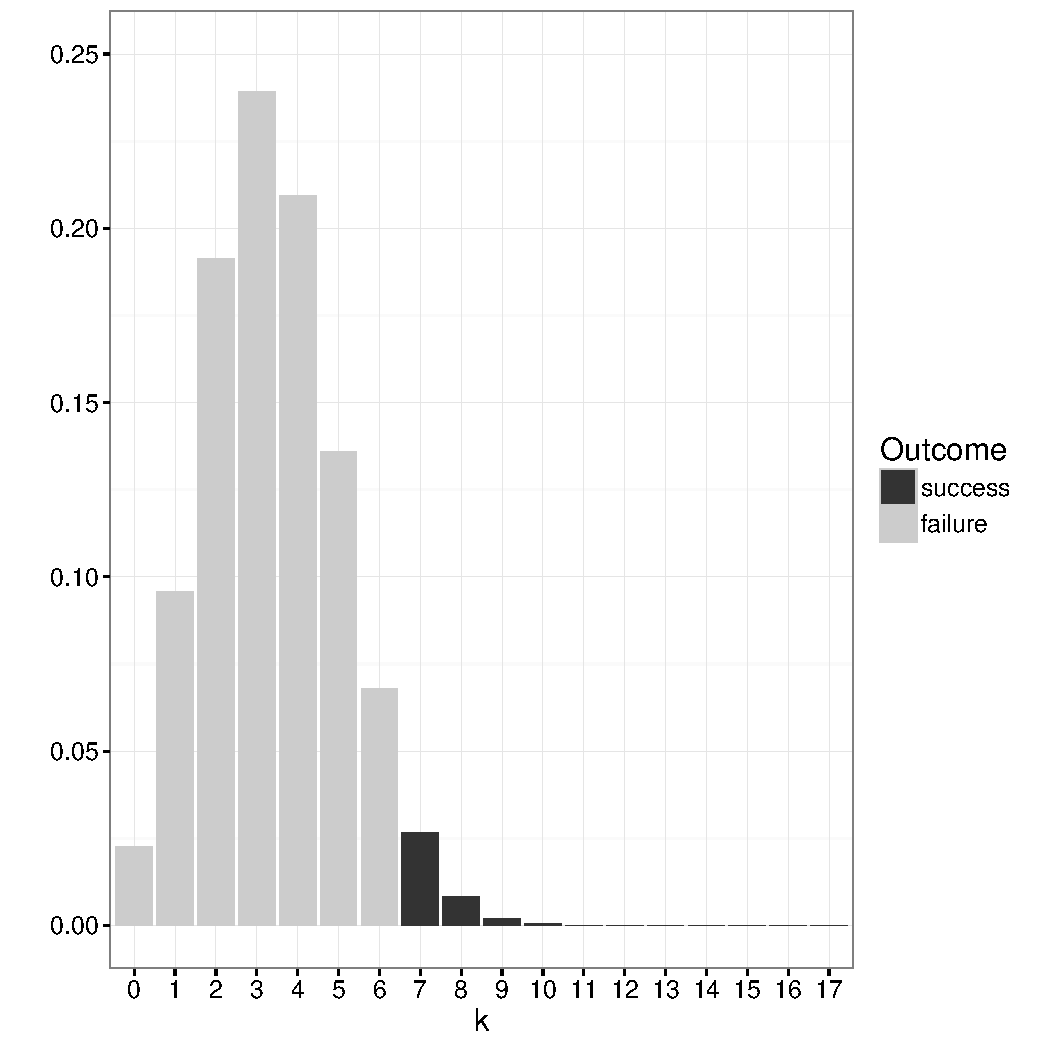
\includegraphics[width=0.5\textwidth]{bin_density.pdf}}
\caption{
SNB(0.2, 7, 11) with mass contributed from 
7 responders (black) or 11 non-responders (grey) along with 
Binomial(0.2, 17) with at least 2 responders (black) or fewer (grey).
}
\label{fig:snb_bin_compare}
\end{figure}

\section{The Moment Generating Function}

The moment generating function for the SNB is calculated in a manner similar to 
that of two negative binomial distributions. 
\begin{prop} Let $Y$ be distributed SNB with parameters $p$, $s$, and $t$.
Then the moment generating function (MGF) of $Y$ is
\begin{equation} \label{eqn:mgf}
\mathbb{E}~e^{xY} = \left(\frac{p e^x}{1 - qe^x}\right)^s 
  \mathcal{I}_{1-qe^x} (s, t) + \left(\frac{qe^x}{1-pe^x}\right)^t 
  \mathcal{I}_{1-pe^x}(t, s)
\end{equation}
for $q = 1-p$ and is defined for 
$x < \min \left\{\log(1/p), \log(1/q) \right\}$.
\end{prop}
\begin{proof}
The MGF of the SNB is:
\begin{equation*}
\mathbb{E}~e^{xY} = \sum_{k=s}^{s+t-1} {k-1 \choose s-1} p^s q^{k-s} e^{kx} 
  + \sum_{k=t}^{s+t-1} {k-1 \choose t-1} p^{k-t} q^t e^{kx}
\end{equation*}
and can be rewritten as:
\begin{equation} \label{eqn:first_sum}
\mathbb{E}~e^{xY} = \sum_{k=s}^{s+t-1}{k-1 \choose s-1} (pe^x)^{s} (qe^x)^{k-s} 
  + \sum_{k=t}^{s+t-1}{k-1 \choose t-1} (qe^x)^t (pe^x)^{k-t}.
\end{equation}
The first summation in (\ref{eqn:first_sum}) satisfies
\begin{align*}
\sum_{k=s}^{s+t-1}{k-1 \choose s-1} (pe)^{sx} (qe^x)^{k-s} &= 
  \left(\frac{pe^x}{1 - qe^x}\right)^s \ \ \sum_{k=s}^{s+t-1} {k-1 \choose s-1} 
    (qe^x)^{k-s} (1-qe^x)^s \\
  &= \left(\frac{pe^x}{1 - qe^x}\right)^s \mathcal{I}_{1-qe^x}(s, t).
\end{align*}
Since the regularized incomplete beta function's subscript parameter 
has support on zero 
to one, we have $0 \leq qe^x < 1$. This implies
$x < -\log(q)$.
A similar expression can be derived for the second summation in 
(\ref{eqn:first_sum}) and results in
the constraint $x < -\log(p)$.
\end{proof}

The SNB's ability to approximate the geometric, normal, gamma, and Poisson
distributions follow from it generalizing the negative binomial distribution. 
\begin{prop}
The MGF of the SNB converges to that of the negative binomial when either
$s$ or $t$ gets large. That is
\begin{equation*}
\mathbb{E} e^{xY} \rightarrow \left( \frac{pe^x}{1-qe^x} \right)^s
\end{equation*}
as $t \rightarrow \infty$. The analogous result holds when 
$s \rightarrow \infty$.
\end{prop}
\begin{proof}
The second regularized incomplete beta term in (\ref{eqn:mgf}) can be written
in terms of a cumulative binomial distribution
\begin{equation*}
\mathcal{I}_{1-pe^x}(t, s) = \mathbb{P}\left[ B \leq s-1 \right]
\end{equation*}
where $B$ is distributed as
Binomial($t-k$, $pe^x$). By Chebychev's inequality %\cite{Hoeffding1963}
it follows that
\begin{equation} \label{eqn:hoeffding}
\mathbb{P}\left[ B \leq s-1 \right] \leq 
  \frac{ (t-k) pe^x (1-pe^x) }{ \left(s - (t-k)pe^x\right)^2 }
\end{equation}
As $t$ gets large $\mathcal{I}_{1-pe^x}(t, s)$ goes to zero
Likewise, $\mathcal{I}_{1-qe^x}(s, t)$ goes
to one. The proof follows by realizing 
\begin{equation*}
0 < \frac{qe^x}{1-pe^x} < 1
\end{equation*}
over the support of $x$.
\end{proof}

When $s=1$ (and $t$ is still large) the SNB's MGF is approximately 
the same as that of the
geometric distribution. The negative
binomial can therefore be seen as a sum of i.i.d. geometric distributions.
For an appropriately large number of samples, the central limit theorem
yields a normal approximation.

Drawing connections to the gamma and Poisson distributions are more complicated.
However a connection to the gamma distribution well-studied problem in the 
literature (see \cite{Ord1968,Guenther1972,Best1974} for examples). 
A connection to the Poisson appears in \cite{Anscombe1950} where
it is shown that if the mean of a Poisson is proportional
to a chi-square distribution with $2k$ degrees of freedom
then the negative binomial is obtained. 
Both of these approximations work by equating cumulants and then showing 
that differences between the cumulant generating
functions converge to zero.

The lower-half normal distribution can be approximated by setting $s=t$
for appropriately large $s$ and $t$ and $p = 0.5$. In this
case, the SNB can be viewed as identical, negative binomials
approximating a normal and truncated at the median.

\section{The Posterior and Predictive Probability Distribution}

Let us consider the case where the rate parameter is distributed 
as Beta($\alpha$, $\beta$) and denoted $P$.
The prior times the likelihood is given by the function
\begin{align} \label{eqn:ptl}
f_P(p, \alpha, \beta ) f_{Y|P}(p, k, s, t) &= 
  \frac{ {k-1 \choose s-1} }{B(\alpha, \beta)} p^{\alpha +s -1} 
    (1-p)^{k+\beta-s-1} + \\
  & \frac{ {k-1 \choose t-1} }{B(\alpha, \beta)} p^{k+\alpha -t -1} 
    (1-p)^{\beta+t-1} \nonumber
\end{align}
where $0 \leq p \leq 1$, $s \leq k \leq s+k-1$, and $t \leq k \leq s+k-1$.
This result can be found directly by multiplying the probability mass function
in (\ref{eqn:pmf}) by the density of the Beta distribution.

The predictive distribution of the SNB can be found by integrating
$p$ over the interval zero to one and applying the definition of the 
beta function.
\begin{align} \label{eqn:predictive}
f_{Y}(k, s, &t, \alpha, \beta) = 
  \int_0^1 f_P(p | \alpha, \beta )  f_{Y|P}(p, k, s, t) dp \nonumber \\ 
 & = {k-1 \choose s-1} \frac{B\left(\alpha+s, k-s+\beta \right)}{B(\alpha, \beta)} 
    + {k-1 \choose t-1} 
    \frac{B\left(\alpha + k - t, t+\beta\right)}{B(\alpha, \beta)}.
\end{align}
If both $\alpha$ and $\beta$ are non-negative integers then the predictive
distribution is a mixture of hypergeometric distributions. 
\begin{align*} \label{eqn:hypergeo}
f_{Y}(k, s, t, \alpha, \beta) = 
  \frac{ {k - 1 \choose s - 1 } 
         {\alpha + \beta \choose \alpha} }{
         {\alpha + \beta + k - 1 \choose \alpha + s}}
  \frac{\alpha}{\alpha + \beta}
  \frac{ \beta }{ k-s+\beta } +
  \frac{ {k - 1 \choose t - 1} 
         {\alpha + \beta \choose \beta} 
         }{
         {\alpha + \beta + k -1 \choose t + \beta}
       }
  \frac{ \beta }{ \alpha + \beta}
  \frac{ \alpha }{ k-t + \alpha}
\end{align*}
The ratio of combinations in the first term can be interpreted as the
probability of $s-1$ responders from $k-1$ patients in $\alpha + s$ draws
from a population size of $\alpha + \beta + k - 1$. This value is multiplied
by $\alpha / (\alpha + \beta)$, the expected response rate of the prior. 
The final term in the product weigths the prior based on the number
of non-responders ($k-s$). Terms in the second summand are interpreted similarly
for non-responders.

The ratio of (\ref{eqn:ptl}) divided by (\ref{eqn:predictive}) gives the 
posterior distribution of $P$. It is a mixture of beta distributions. The
mixing parameter depend on the endpoints ($s$ and $t$), the number of enrollees needed to reach an endpoint ($k$), and the prior parameters ($\alpha$ and
$\beta$).

\begin{figure}[t!]
\centering
\includegraphics[width=\textwidth]{beta-mixture.pdf}
\caption{
The posterior distribution of the response probability with 
the Jeffreys prior ($\alpha=\beta=1/2$) for the trial where
$s=7$, $t=11$, $k=15$.
}
\label{fig:beta_mixture}
\end{figure}

The posterior result above is for the case where the parameters are known
and the endpoint is not. That is, we do not which boundary was reached.
Fig.~\ref{fig:beta_mixture} shows this distribution based on the 
parameters in the hypothetical trial assuming the
Jeffreys prior \citep{Jeffreys1946}.  If we include the fact that the
trajectory reaches the endpoint then the second terms in (\ref{eqn:ptl}) and
(\ref{eqn:predictive}) are both zero and the posterior distribution is
Beta(7.5, 8.5). This is proportional to the area labeled ``success'' in 
Fig.~\ref{fig:beta_mixture}.

%\begin{proof}
%For notational simplicity, assume that $k$ is in the range
%$\min(s,t) \leq k \leq s+t-1$. When 
%this is not the case appropriate terms should be removed as dictated by the indicator functions.
%\begin{align*}
%f(k | s, t, \alpha, \beta) = \frac{1}{B(\alpha, \beta)} & \int_0^1 {k-1 \choose s-1} p^{\alpha +s -1} \left(1-p\right)^{k-s+\beta-1} + \\
% & {k-1 \choose t-1} p^{k-t+\alpha-1}\left(1-p\right)^{t+\beta-1} dp \\
%= \frac{1}{B(\alpha, \beta)}  {k-1 \choose s-1} & \int_0^1  p^{\alpha +s -1} \left(1-p\right)^{k-s+\beta-1} dp + \\
% & \frac{1}{B(\alpha, \beta)} {k-1 \choose t-1} \int_0^1  p^{k-t+\alpha-1}\left(1-p\right)^{t+\beta-1} dp.
%\end{align*}
%The result in (\ref{eqn:posterior}) follows by the definition of the 
%beta function.
%\end{proof}

%To better understand the predictive distribution, let us once again return to 
%our example where $s=7$, $t=11$. However, we assume $p$ has a beta distribution
%with shape parameters $\alpha = 0.2 c$ and $\beta = 0.8 c$ for any $c > 0$.
%This parameterization has mean 0.2 for all $c > 0$ and variance 
%$0.16 / (c+1)$.
%
%
%\begin{figure}[h!]
%\centering
%\subfloat[mean]{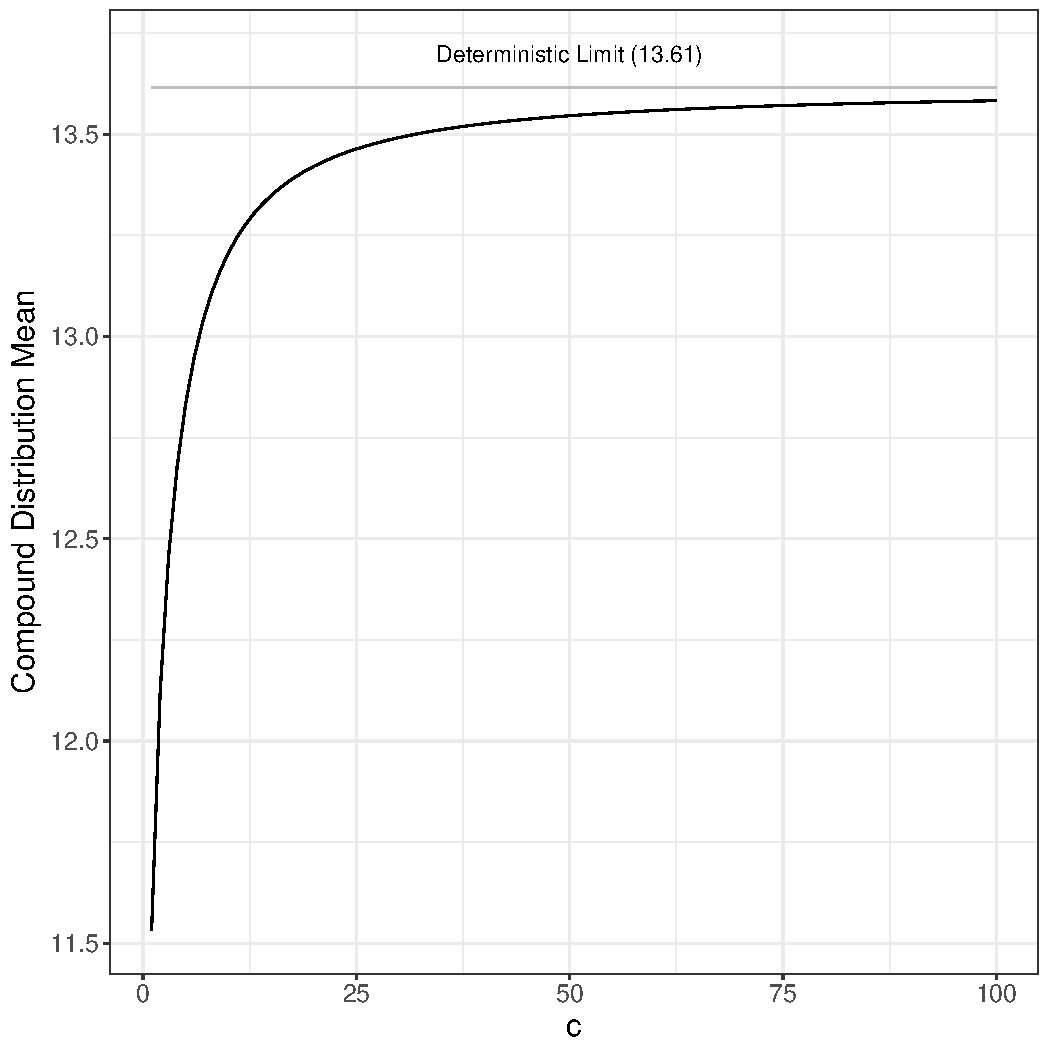
\includegraphics[width=0.5\textwidth]{bayesian-sample-expectation.pdf}}
%\hfill
%\subfloat[variance]{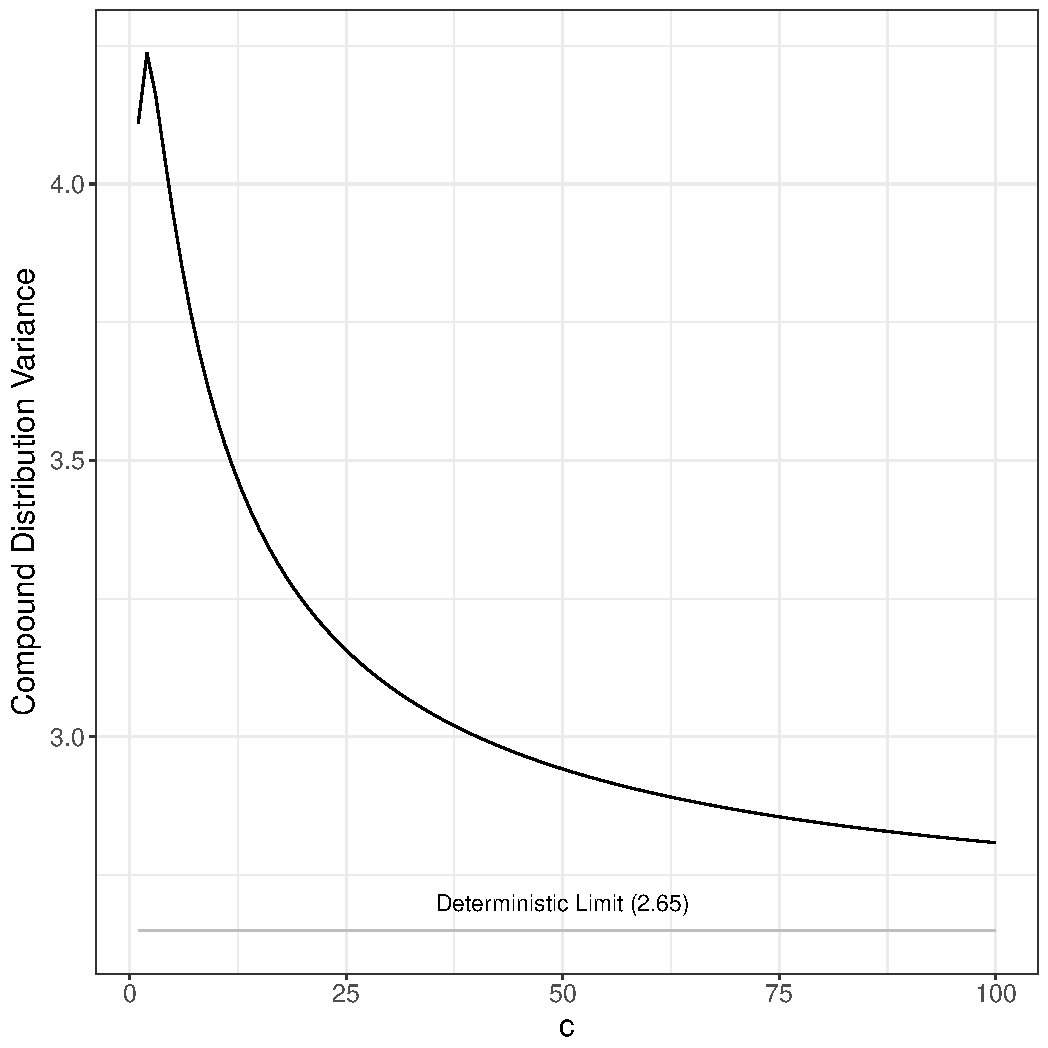
\includegraphics[width=0.5\textwidth]{bayesian-sample-variance.pdf}}
%\caption{
%The mean and variance of the predictive SNB with $s=7$, $t=11$
%with $\mathbb{E}\ p = 0.2$ varying the uncertainty 
%in the distribution of $p$. A larger value of $c$
%corresponds to a beta variance.
%}
%\label{fig:bayesian-sample-size}
%\end{figure}

%As $c$ increases the 
%predictive distribution sample statistics converge to corresponding 
%statistics for the SNB with $p = 0.2$. 
%For estimation it may be 
%preferable to select shape parameters based on the median or mode of the 
%beta distribution since they are less sensitive to distributional uncertainty.

%%It may be noted that the compound 
%%distribution's mean
%%approaches the deterministic limit slowly. This
%%is because when $c$ is small, the distribution of $p$ is heavily skewed. 
%%As $c$ increases this effect is minimized.
%When the distribution of $p$ is centered close to zero or one the mean 
%estimate approach the deterministic limit relatively slowly in the uncertainty
%parameter $c$.  
%\section{Discussion}
%
%The SNB can be used to extend clinical trial methodology
%in at least two areas. First, it can be used to construct nested criteria
%for early stopping and efficacy. Current approaches are often inspired by
%the Simon 2-stage Phase II clinical trial \cite{Simon1989} where a
%a small number of patients are enrolled for an initial stage. For patients,
%success or failure is assessed. If at least a pre-specified number of
%successes are observed then the trial enters a second stage with more
%patients. If a sufficient number of successes are not observed then the
%trial fails. 

%The SNB is being used to generalize the Simon design by providing separate
%criteria for futility and efficacy.
%The Simon design tests for a single response probability and time-to-event
%parameter for both the first
%and second stage. The SNB is being used to generalize this design by 
%allowing these parameters to vary for the two stages, and even allow
%information about patients in the first stage to be used in the second
%stage. Early results show the design provides
%both early testing for futility along with the ability
%to make statistically sound decisions sooner than traditional trials.

%A second avenue for methodological innovation comes directly from
%Corollary \ref{conditional_distribution} and Proposition \ref{prop:bayesian}.
%Our knowledge of the response probability $p$ comes from published reports
%yielding a prior distribution.
%While a trial is being conducted the response probabilities are 
%updated as new results are received. The number of individual successes
%and failure are used to learn the shape characteristics of the corresponding
%beta distribution and resulting posterior
%distribution. An estimate of the probability of reaching the success (and
%failure) endpoints can be provided at each step of the trial.

%There are also several avenues for extending the SNB itself. First is the 
%development of a stopped negative multinomial distribution allowing
%for more than two endpoints. This extension would have clinical trial
%applications including dose escalation where the outcomes are response
%to a therapy, failure to respond, and an adverse outcome endpoint where
%an enrollee is removed from the trial with neither response or non-response
%due to side effects.

%A second, more theoretical extension is to the asymptotic setting. Under
%proper reparameterization, the process from which the SNB is derived 
%can be shown to converge to a Brownian motion. In this case, we conjecture
%that the SNB can be defined in terms of the L\'{e}vy-Bachelier 
%\citep{Bachelier1900} formula
%thereby relating the SNB to the classic result in stochastic calculus.

\section*{References}

\bibliography{mybibfile}

\end{document}
